\section{Results and Discussion}
\label{Results and Discussion}

This section presents the main results for the comparison between the three psychometric instruments. 

\textbf{Personality Test Results}. We obtained personality traits’ scores for each participant by applying the three psychometric instruments (i.e., BFI, 16PF, and CC). It is worth mentioning that each instrument provided a set of personality trait scores for each participant. We calculated these scores using the guidelines for each instrument. Next, we present the results when applying each psychometric instrument.

\textit{BFI results:} We found the following quantities of participants with the dimension value assessed above 50\%: Extraversion (20 participants), Agreeableness (29 participants), Conscientiousness (28 participants), Neuroticism (12 participants), and Openness to Experience (24 participants). 

\textit{16PF results:} We found more Extroverts (52\%) types than Introverts (48\%), more Sensing (55\%) than Intuitive (45\%), fairly more Feeling (65\%) than Thinking (35\%), and more Judging (65\%) compared to Perceiving (35\%) type. The personality types most present were ENFJ, ESFJ, and ISFJ. However, we did not have participants with the personality types ISTP, ESTP, INFJ, and ENTP. Considering the Identity scale, the personality type most present was ENFJ-A.

\textit{CC results:} We obtained the following quantities of participants with the factor value assessed above 50\%: Extraversion (17 participants), Agreeableness (27 participants), Conscientiousness (15 participants), Neuroticism (4 participants), and Openness to Experience (8 participants). 

We analyzed the number of questions, option type, and time to respond to the psychometric instruments compared. Considering the number of questions and option type, 16PF contains 60 7-point questions, BFI-44 contains 44 5-point questions, and CC contains 44 A or B questions. The participant's average response time was 12 minutes to 16PF, 10 minutes to BFI-44, and 15 minutes to CC. 

Nevertheless, in addition to these comparison criteria, we were interested in the correlation between the test results (i.e., the correlation between the facets, dimensions, and aspects of psychometric instruments). We discussed the analysis of this criterion by answering the research questions.

\textbf{RQ1 - To what extent do BFI dimensions correlate with 16PF aspects considering software developers’ personality?}. Aims to address this RQ, we applied Kendall’s correlation between 16PF dichotomies and BFI dimensions. The correlation results can be seen in Table~\ref{tabela3}.

\begin{table}[!h]
\centering
\caption{Correlation between 16PF Dichotomies
 and BFI Dimensions.}
\label{tabela3}
\scalebox{0.80}{
\begin{tabular}{c|ccccc|}
\cline{2-6}
\multicolumn{1}{l|}{}                    & \multicolumn{5}{c|}{\textbf{BFI}}                                                        \\ \cline{1-1}
\multicolumn{1}{|c|}{\textbf{16PF}}      & \textbf{Extrav.} & \textbf{Agree.} & \textbf{Openn.} & \textbf{Consc.} & \textbf{Neuro.} \\ \cline{2-6} 
\multicolumn{1}{|c|}{\textbf{Extrovert}} & \text{0.57}    & 0.23            & 0.29            & 0.40            & -0.17           \\ \cline{2-6} 
\multicolumn{1}{|c|}{\textbf{Feeling}}   & 0.04             & \text{0.53}   & -0.08           & 0.13            & -0.19           \\ \cline{2-6} 
\multicolumn{1}{|c|}{\textbf{Intuitive}} & 0.01             & -0.03           & \text{0.50}   & -0.27           & -0.05           \\ \cline{2-6} 
\multicolumn{1}{|c|}{\textbf{Judging}}   & 0.12             & 0.11            & -0.12           & \text{0.71}   & -0.08           \\ 
\cline{2-6} 
\multicolumn{1}{|c|}{\textbf{Assertive}} & 0.33    & 0.24            & 0.15            & \text{0.40}            & \text{-0.57}           \\
\hline
\end{tabular}}
\end{table}

Figure~\ref{fig2} shows the distribution of participants considering the 16PF's Extroversion dichotomy (16PF-E), 16PF's Introversion dichotomy (16PF-I), and the  BFI's Extraversion dimension (BFI-E). In the figure, each point represents the participant score (i.e., the score of dimension or facet) obtained from the psychometric instrument.

\begin{figure}[!ht]
\centerline{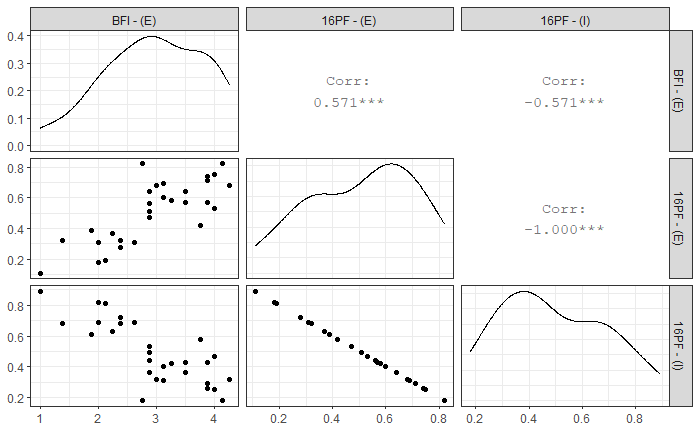
\includegraphics[scale=0.40]{Imagens/n1.PNG}}
\caption{The correlation coefficient between 16PF's Extroversion dichotomy (16PF-E), 16PF's Introversion dichotomy (16PF-I), and BFI's Extraversion dimension (BFI-E).}
\label{fig2}
\end{figure}

We found a moderate correlation between BFI's Extraversion dimension (BFI-E) and the 16PF's Mind aspect (16PF-E and 16PF-I). This correlation was positive to 16PF's Extroversion dichotomy (16PF-E) and negative to 16PF's Introversion dichotomy (16PF-I). The coefficient of 0.571 (p $<$  0.01) indicates a moderate positive correlation between 16PF-E and BFI-E. As expected, the correlation for 16PF-I was inversely correlated -0.571 (p $<$  0.01) with BFI-E. The results found reinforced the analysis performed by Jia et al.~\cite{jia2015comparative, balijepally2006assessing}, which stated that BFI's Extraversion dimension (BFI-E) is correlated to the 16PF's Extroversion dichotomy (16PF-E). 

%\begin{table}[http]
%\centering
%\caption{Personality Assessment Methods}
%\label{tabela1}
%\scalebox{0.70}{
%\begin{tabular}{|c|c|c|c|}
%\hline
 %                     & \textbf{\begin{tabular}[c]{@{}c@{}}Number\\ of questions\end{tabular}} %& \textbf{Option type}                                    & %\textbf{\begin{tabular}[c]{@{}c@{}}Average \\response time\end{tabular}} \\ \hline
%\textbf{16PF}          & 60                                                                    & %\begin{tabular}[c]{@{}c@{}}7-point\\ scale\end{tabular} & 12 minutes                                                            \\ \hline
%\textbf{BFI-44}  & 44                                                                     & %\begin{tabular}[c]{@{}c@{}}5-point\\ scale\end{tabular} & 10 minutes                                                             \\ \hline
%\textbf{Context Cards} & 60                                                                     %& A or B                                                  & 15 minutes                           %                                 \\ \hline
%\end{tabular}}
%\end{table}

Considering the distribution of participants for 16PF's Feeling dichotomy (16PF-F) and 16PF's Thinking dichotomy (16PF-T) and the BFI's Agreeableness dimension (BFI-A), We found a moderate correlation with a coefficient of 0.534 (p $<$ 0.01) between 16PF-F and BFI-A. As expected, the correlation between 16PF-T and BFI-A was inversely correlated. Also, we found a moderate correlation between BFI's Conscientiousness dimension (BFI-C) and the 16PF's Identity aspect. This correlation was positive to 16PF's Assertive dichotomy (16PF-A) and negative to 16PF's Turbulent dichotomy (16PF-T).

Similarly, we obtained a moderate correlation between BFI's ``Openness to Experience'' dimension (BFI-O) and the 16PF's Energy aspect (16PF-N and 16PF-S). This correlation was positive to 16PF's Intuitive dichotomy (16PF-N) and negative to 16PF's Observant dichotomy (16PF-S). The correlation coefficient of 0.502 (p $<$ 0.01) indicated a moderate correlation between the BFI-O and the 16PF's Intuitive dichotomy (16PF-N). As expected, the correlation coefficient was negative between the BFI's ``Openness to Experience'' dimension (BFI-O) and the 16PF's Observant dichotomy (16PF-S).  

Considering the 16PF's Judging dichotomy (16PF-J), 16PF's Prospecting dichotomy  (16PF-P), and the BFI's Conscientiousness dimension (BFI-C). The correlation coefficient of 0.712 (p $<$ 0.01) indicated a strong positive correlation between 16PF-J and BFI-C. As expected, the correlation between 16PF-P and BFI-A was inversely correlated -0.712 (p $<$ 0.01). We obtained a strong correlation between BFI-C and the 16PF's Tactic aspect (16PF-J and 16PF-P). This correlation was positive with 16PF-J and negative to 16PF-P.  

As in previous studies ~\cite{cattell2008sixteen,cattell1995personality, schneewind199816, gerbing199116pf} our study identified a strong correlation between 16PF-J and BFI-C.  However, we found a moderate correlation between 16PF-E and BFI-E, 16PF-F and BFI-A, and 16PF-N and BFI-O, unlike Cattell and Mead ~\cite{cattell2008sixteen}, which found a strong correlation. Additionally, we observed a weak correlation between 16PF-F and BFI-N. 

Further, we analyzed the correlation of 16PF's Identify aspect (16PF-A and 16PF-T) with BFI's dimensions. We obtained a coefficient of -0.578 (p $<$ 0.01) for the correlation between the 16PF's Assertive dichotomy (16PF-A) and BFI's Neuroticism dimension (BFI-N). Further, the correlation between (16PF-A) and BFI's Conscientiousness dimension (BFI-C) was 0.40 (p $<$ 0.01). Considering the 16PF's Turbulent dichotomy (16PF-T), we obtained a correlation coefficient of 0.580 (p $<$ 0.01) with BFI-N, and -0.416 (p $<$ 0.01) with BFI-C. Table~\ref{tabela3} illustrates the results of Kendall’s correlation between 16PF dichotomies and BFI dimensions. 
 
We concluded that BFI-C correlated strongly with 16PF-E. We found a moderate correlation between 16PF-E and BFI-E, 16PF-F and BFI-A, and 16PF-N and BFI-O. We found a weak correlation between 16PF-F and BFI-N. Further, 16PF-A correlated moderately with BFI-C (moderately positive) and BFI-N (moderately negative). Thus, we concluded that BFI and 16PF had a moderate correlation. 


\textbf{RQ2 - To what extent do 16PF aspects correlate with CC factors considering software developers’ personality?}.
Aims to address this RQ, we applied Kendall’s correlation between 16PF dichotomies and CC factors. The correlation results can be seen in Table~\ref{tabela45}. The correlation coefficient of 0.35 (p $<$  0.01) indicates a weak positive correlation between 16PF's Extroversion dichotomy (16PF-E) and the CC's Extroversion factor (CC-E). Additionally, we obtained a weak correlation between 16PF's Mind aspect (16PF-E and 16PF-I) and CC's Extroversion factor (CC-E).
Similar to what happens with 16PF and BFI.

\begin{table}[!ht]
\centering
\caption{Correlation between 16PF Dichotomies and context cards factors.}
\label{tabela45}
\scalebox{0.80}{
\begin{tabular}{c|ccccc|}
\cline{2-6}
\multicolumn{1}{l|}{}                    & \multicolumn{5}{c|}{\textbf{Context Cards}}                                              \\ \cline{1-1}
\multicolumn{1}{|c|}{\textbf{16PF}}      & \textbf{Extrav.} & \textbf{Agree.} & \textbf{Openn.} & \textbf{Consc.} & \textbf{Neuro.} \\ \cline{2-6} 
\multicolumn{1}{|c|}{\textbf{Extrovert}} & \text{0.35}    & 0.09            & -0.036          & -0.21           & 0.10            \\ \cline{2-6} 
\multicolumn{1}{|c|}{\textbf{Feeling}}   & 0.11             & 0.07            & 0.09            & -0.25           & \text{-0.34}  \\ \cline{2-6} 
\multicolumn{1}{|c|}{\textbf{Intuitive}} & 0.007            & -0.14           & 0.25            & -0.09           & 0.02            \\ \cline{2-6} 
\multicolumn{1}{|c|}{\textbf{Judging}}   & 0.19             & 0.14            & \text{-0.36}  & -0.008          & 0.05            \\ 
\cline{2-6} 
\multicolumn{1}{|c|}{\textbf{Assertive}} &0.29    & 0.27            & 0.02            & \text{-0.33}            & -0.08          \\
\hline
\end{tabular}}
\end{table}

Regarding 16PF's Judging dichotomy (16PF-J) and CC's ``Openness to Experience'' factor (CC-O), we found a negative correlation -0.36 (p $<$  0.01) between 16PF-J and CC-O.  Further, we found a weak correlation between CC's ``Openness to Experience'' factor (CC-O) and the 16PF's Tactic aspect (16PF-J and 16PF-P. Considering the 16PF's Feeling dichotomy (16PF-F) and CC's Neuroticism factor (CC-N), we observed a negative correlation coefficient of -0.34 (p $<$ 0.01), which indicated the weak correlation between these characteristics. Finally, we found a weak correlation between CC's Neuroticism factor (CC-N) and 16PF's Nature aspect (16PF-T and 16PF-F). Given the discussed results, we concluded that the correlation between 16PF and CC was weak.

\textbf{RQ3 - To what extent do BFI dimensions correlate with CC factors considering software developers’ personality?}. Aiming to address this RQ, we applied Kendall’s correlation between BFI dimensions and CC factors. The correlation results can be seen in Table~\ref{tabela5}. Considering the five characteristics analyzed for each psychometric instrument, we had a weak correlation (correlation coefficient of 0.38 (p $<$ 0.01)) between CC's Extroversion factor (CC-E) and BFI's Extraversion dimension (BFI-E). We found a correlation coefficient of 0.30 (p $<$ 0.01) between BFI's Conscientiousness dimension (BFI-C) and CC's Extroversion factor (CC-E). Further, we obtained a weak correlation between CC's Extroversion factor (CC-E) and the BFI's Extraversion dimension (BFI-E). 
CC's Conscientiousness factor (CC-C) had a correlation coefficient of -0.34 (p $<$ 0.01) with BFI's Agreeableness dimension (BFI-A) and 0.32 (p $<$ 0.01) with BFI's Neuroticism dimension (BFI-N). Thus, we concluded that there was a weak correlation between CC's Conscientiousness factor (CC-C) and the BFI's Agreeableness dimension (BFI-A) and BFI's Neuroticism dimension (BFI-N).  


\begin{table}[!ht]
\centering
\caption{Correlation between BFI Dimensions and context cards factors.}
\label{tabela5}
\scalebox{0.80}{
\begin{tabular}{c|ccccc|}
\cline{2-6}
\multicolumn{1}{l|}{}                  & \multicolumn{5}{c|}{\textbf{Context Cards}}                                              \\ \cline{1-1}
\multicolumn{1}{|c|}{\textbf{BFI}}     & \textbf{Extrav.} & \textbf{Agree.} & \textbf{Openn.} & \textbf{Consc.} & \textbf{Neuro.} \\ \cline{2-6} 
\multicolumn{1}{|c|}{\textbf{Extrav.}} & \text{0.38}    & 0.04            & -0.02           & -0.21           & 0.002           \\ \cline{2-6} 
\multicolumn{1}{|c|}{\textbf{Agree.}}  & 0.28             & 0.27            & -0.09           & \text{-0.34}  & -0.30           \\ \cline{2-6} 
\multicolumn{1}{|c|}{\textbf{Openn.}}  & 0.15             & -0.08           & 0.12            & -0.21           & 0.19            \\ \cline{2-6} 
\multicolumn{1}{|c|}{\textbf{Consc.}}  & \text{0.30}    & -0.08           & -0.21           & -0.09           & 0.04            \\ \cline{2-6} 
\multicolumn{1}{|c|}{\textbf{Neuro.}}  & -0.12            & -0.24           & -0.02           & \text{0.32}   & 0.16            \\ \hline
\end{tabular}}
\end{table}


Despite measuring similar characteristics, we concluded that the relationship between BFI and CC is weak. These results are not similar to those found by Yilmaz at el.~\cite{yilmaz2017examination}, in which the authors proposed and validated CC. In this study, they proposed results that assumed a strong correlation between the use of CC and BFI. Such correlations were the CC's Extroversion factor (CC-E) with the BFI's Extraversion dimension (BFI-E) (correlation coefficient of 0.93). They also found a strong correlation between CC's Conscientiousness factor (CC-E) and BFI's Conscientiousness dimension (correlation coefficient of 0.79).

We believe that a possible explanation for such distinction between the study findings and Yilmaz et al.'s~\cite{yilmaz2017examination} maybe the loss of semantics aspects from the original CC (once the originals were written in English language and the ones applied here were translated into Brazilian Portuguese). Besides that, the cultural factor may have influenced the interviewees' understanding of some questionnaire items' situations. We concluded that CC inventory is currently lacking independent replications to validate its reliability. In sum, this highlights the importance of developing such research in the SE field to enhance the surveys and studies that approach psychometric aspects and team formation. 











































